\documentclass[a4paper]{article}
\usepackage[bottom=2.5cm]{geometry}
\usepackage[table]{xcolor}
\usepackage{graphicx}
\usepackage{sectsty} %to customise headings
\usepackage{times} %this is for the selection of font
\usepackage{fancyhdr}	
\usepackage[ampersand]{easylist}
\usepackage{amssymb}
\usepackage{enumitem}	
\usepackage{tabu}
\usepackage{longtable}
\usepackage{booktabs}
\usepackage{eso-pic}
\usepackage{transparent}
\usepackage{pdfpages}

\usepackage{ltablex}
\setlength{\LTpre}{0pt}
\setlength{\LTpost}{-15pt}

\usepackage{array}
\usepackage{tabularx}
\usepackage{pgfplots, pgfplotstable}

\usetikzlibrary{backgrounds}
% background color definition from pgfmanual-en-macros.tex
\definecolor{graphicbackground}{cmyk}{0.04,0.02,0.02,0.04}
% key to change color
\pgfkeys{/tikz/.cd,
	background color/.initial=graphicbackground,
	background color/.get=\backcol,
	background color/.store in=\backcol,
}
\tikzset{background rectangle/.style={
		fill=\backcol,
	},
	use background/.style={    
		show background rectangle
	}
}


	
\pagestyle{fancy}
\lhead{Implementation of Onboarding Document Tool}
\cfoot{\scriptsize{Thrymr Software Pvt. Ltd.\\Contact@thrymr.net \quad Call Us : 040-64550008\\ }}
% Set the right side of the footer to be the page number
\fancyfoot[R]{\thepage}
\renewcommand{\headrulewidth}{0.4pt}
\renewcommand{\footrulewidth}{0.4pt}

\usepackage{lipsum}% Used for dummy text.

\definecolor{titlepagecolor}{cmyk}{1,.60,0,.40}
\definecolor{namecolor}{cmyk}{1,.50,0,.10} 
\definecolor{levelfirst}{cmyk}{0.2,1,0.55,0.70}
\definecolor{levelSecond}{cmyk}{1,.50,0,.10}
\definecolor{levelthird}{cmyk}{1,.50,0,.10}
\definecolor{levelfourth}{cmyk}{1,.50,0,.10}
\definecolor{levelfifth}{cmyk}{1,.50,0,.10}

\definecolor{tablecell1}{cmyk}{0.07,0.03,0.03,0.07}
\definecolor{tablecell2}{cmyk}{0.04,0.02,0.02,0.04}
%-----------------------------------------------------------------
\begin{document}
	% ----------------------------------------------------------------
	\begin{titlepage}
	\iffalse   % iftrue fr display, iffalse to hide display
	
		\newgeometry{left=3.5cm, bottom=2cm} %defines the geometry for the titlepage
		\pagecolor{titlepagecolor}
		\noindent
		\includegraphics[width=6cm]{allegis2.jpg}\\[-1em]
		\color{white}
		\makebox[0pt][l]{\rule{1.3\textwidth}{1pt}}
		\par
		\noindent
		\textcolor{namecolor}{\Huge{\textbf{Proposal for the Implementation of\\ \\}}}
		\noindent\textbf{\Huge \textsf{Onboarding Document Tool\\ \\}} 
		\noindent\textsf{October 2015}
		\vfill
		\vskip\baselineskip
		\noindent
		\includegraphics[width=6.4cm]{Logo.png}\\[1em]
		{\textsf{Thrymr Software Pvt. Ltd\\}}
		{\textsf{Center for Innovation and Entrepreneurship\\Vindhya C-4 IIIT-Campus \\ Gachibowli, Hyderabad \\ Telangana State, India\\ \\ \\}}
		\textcolor{namecolor}{\small{\textbf{Statement of Confidentiality\\} \\\textcolor{namecolor}{\footnotesize{This data shall not be disclosed and shall not be duplicated, used, or disclosed in whole or in part for any purpose. If a contract is awarded to Thrymr Software, as a result of or in connection with the submission of this data, the client or prospective client shall have the right to duplicate, use, or disclose this data to the extent provided in the contract. This restriction does not limit the client’s or prospective client’s right to use the information contained in the data if it is obtained from another source without restriction. The data subject to this restriction is contained in all marked sheets.}}}}\noindent
		
		\noindent
	\fi
	
	\includepdf[titlepages={}]{TitlePage2.pdf}
		
	\end{titlepage}
	\restoregeometry % restores the geometry
	\nopagecolor % Use this to restore the color pages to white
	% ----------------------------------------------------------------
	\tableofcontents
	\setcounter{tocdepth}{2}
	
	
	\newpage
	
	\linespread{1.3}
	
	\newcommand\BackgroundPic{
		\put(-3,-0.5){
			\parbox[b][\paperwidth]{\paperheight }{%
				\vfill
				%\centering
				{\transparent{0.4} \includegraphics[width=\paperheight, keepaspectratio ]{Pagelayout1.jpg}}%
				\vfill
			}}
			\put(0,4){%
				\transparent{0.4}\textcolor{white}{\rule{\paperwidth}{\paperheight}}
			}
			}
			
	\AddToShipoutPicture{\BackgroundPic}		
	\sectionfont{\color{levelfirst}}
	\section{Executive Summary}
	
	\subsectionfont{\color{levelfirst}}
	\subsection{The Website and Mobile Application Development Process}
	Time and again studies have shown the positive impact Websites and mobile applications have on business. At Thrymr we create Websites and Mobile applications in a cost effective manner based on budget and design. These applications can be made compatible for the iPhone and Android systems. We partner you in creating websites and mobile applications at critical stages of the entire process; from designing, to writing code, to test runs.
	
	\subsection{Improving Business Workflows} %or Marketing your Business
	Websites have a wider reach and help to showcase your products and services to a wider audience.  A dynamic and vibrant website will function as a bridge between the clients and the products. The website is absolutely the best way to demonstrate the efforts your company is taking to better serve the existing customers and attract new ones.
	Mobile applications have allowed businesses to become convenient and inclusive to the needs and demands of the consumer. A business can provide internal stakeholders with mobile applications for business workflows and data capture. Also applications increasingly are serving the variety of different services, internal and external that a business needs to function.
	
	\subsection{Cutting Costs and Profitability}
	In order for businesses to be competitive in the market, the need for increased efficiency arises within each industry in order to compete within each market. Technology within each market provides these industries the outlet for businesses to decrease costs and in turn increase the profitability of the business. Along with websites most recently, the rise of mobile interface and the application that come with it give a new facet for businesses to increase their efficiency.
	
	\subsection{Other Advantages}
	Websites and Mobile applications are speeding up the business world, allowing for products and services along with business strategies and plans to be available to consumers and business users at the touch of a button. Large databases of information and files can now be stored online and accessed at any given time with new technology.  Finally, mobile applications enhance productivity as they allow for Business Users to access a business’s services and products and for brands to market themselves to consumers and interact with them in real time.  Ultimately, with enhanced customer satisfaction and more rapid problem-solving technology and organizational tools, websites and mobile applications allow for businesses to obtain more revenue in the long run.
	
	\newpage
	
	\section{Company Overview}
	
	\subsection{About Thrymr Software}
	Started in early 2013, Thrymr Software is a software product company. Founded by IITians, Thrymr excels in design and development of software products for both web and mobile platforms. Whether it is building great software products for ourselves or our clients, we bring in loads of passion and dedication to our work. Our vision is to be the best-in-class provider of software products.
	We pride ourselves in building top of the line cloud-based software using HTML5, Java, Play Framework and PostgreSQL.
	Thrymr has had immense experience in development of web and mobile application for clients cutting across domains and sectors ranging from financial to health care.
	
	\subsection{Our Products \& Services}
	
	\textbf{Software Development:} {Leave it to us to deliver world-class software with great quality, on-time and within budget.\\ \\}
	{MedNetwork developed by Thrymr aims to revolutionize the way healthcare is delivered. With online, cloud based platform, MedNetwork makes healthcare delivery smart, fast, integrated and efficient for all the stakeholders involved.\\ \\}
	\textbf{Mobile Application Development:} {Great mobile apps that are responsive, focussed on your market and aesthetically beautiful. That's what we deliver for you!.\\ \\}
	\textbf{Design Services:} {From conceptualisation to Prototyping to final delivery, rely on us to deliver outstanding designs for your software products and websites.\\ \\}
	\textbf{Enterprise Application Development:}{From complex ecosystems to simple solutions, we partner with you to develop an integrated and wholesome software that takes care of end-to-end needs of your organisation.}
	
	\subsection{Our Clients}
	
	\bigskip
	\includegraphics[ width=\textwidth , keepaspectratio ]{Client.png}\\[-1em]
		
	\newpage
	
	\section{Scope Definition}
	The Admin module of the application shall be a web-based deployment. The User module shall be a website with mobile and desktop versions. The high level functional requirements are as below:
	
	\subsection{Web based Administration Module}
			
	\ListProperties(Hide=100, Hang=true, Progressive=6ex, Space=0.8em,Space*=0.8em, Style*=$\bullet$, Style2*=$\bullet$ ,Style3*=$\bullet$ ,Style4*=\tiny$\blacksquare$ )
	
	
	\begin{easylist}
		& \thinspace Manage Job IDs
		&& Create Job Category
		&&& Create Job ID
		& \thinspace  Modify Job Category
		&& Modify Job ID
		& \thinspace  Upload Facility
		& \thinspace  Deactivate Job Category
		&& Deactivate Job ID
		& \thinspace  Remove Job Category
		& \thinspace  User Registration / Create User
		&& Select User Type ( Admin-Normal/ Admin- Subuser / Candidate/ Employee)
		&& Select Job ID offered (not applicable for Admin)
		& \thinspace  Modify User
		&& Modify Admin User
		&& Modify Candidate User Type  and Details (only from Candidate to Employee, not vice-versa)
		&&& Generate User ID and Password 
		&&& Send Notifications
		&&& Clone and/or Create documents folder
		&& Activate/ Deactivate User
		&& Remove User
		& \thinspace Dashboard/ Manage Onboarding Process
		&& View New Candidates/ Users
		&&& Send Invite to Candidates for registration
		&& View Registered Candidates
		&&& View ‘Pre-join’ Submit Status
		&&& Auto-Download forms to set path
		&&& View Documents
		&&& Approve / Reject 
		&&& On Approve Automatically “Modify” user type and send “employee invite”
		&& View Employee
		&&& Send Employee Invite
		&&& View ‘Post-Join’ Submit Status
		&&& Auto-Download forms to set path
		&&& View Documents
		&& Client Management
		&&& Create Client
		&&& Modify Client
		&&& Activate / Deactivate Client
		&&& Remove Client
		& \thinspace Session Management
		& \thinspace Authentication Features and control
		& \thinspace Broadcast / Send notifications
		& \thinspace Reporting 
		& \thinspace Account Settings
		
		
	\end{easylist}
		
	\subsection{Website - Candidate/ Employee Module }
	
	\begin{easylist}
		& \thinspace Candidate/ Employee Sign-on
		& \thinspace Retrieve Credentials
		& \thinspace Initiate ‘Pre-Joining’
		&& Application form
		&&& Client Name/ Client Location/ Photo
		&&& Personal Details
		&&& Residential Address
		&&& Educational Details
		&&& Employment Details
		&&& Personal References
		&&& Declaration
		&& Bank Information
		&& Family Particulars
		&& Form 1 - Nomination and Declaration Form
		&&& View
		&&& Edit fields
		&&& Preview and Submit
		&&& Download
		&& Form F - Payment of Gratuity
		&&& Build Automatically
		&&& Edit fields
		&&& Preview and Submit
		&&& Download
		&& Form Q - Appointment Order
		&&& Build Automatically
		&&& Edit fields
		&&& Preview and Submit
		&&& Download
		&& Form 2 and Declaration Form - EPF and Pension Scheme
		&&& Build Automatically
		&&& Edit fields
		&&& Preview and Submit
		&&& Download
		&& Form XIII
		&&& Build Automatically
		&&& Edit fields
		&&& Preview and Submit
		&&& Download
		&& Any Other Documents
		&&& Description field + Upload
		& \thinspace Post-Join formalities (only available for Employee Login)
		&& View Offer Letter
		&& Accept Offer Letter
		& \thinspace Account Settings
		& \thinspace View Notifications
		
		
	\end{easylist}
	
	\subsection{Interfaces }
	
	\begin{easylist}
		& \thinspace File Server
		& \thinspace Report Server
		
	\end{easylist}
	
	\subsection{Reporting Management (Integrated with Web-based Admin Module) }
		
	\begin{easylist}
		& \thinspace User reports
		&& Login/ Logout/ Session Timeout
		& \thinspace Onboarding Statistics
		& \thinspace Reports by various attributes like Candidate, Role, Client etc
			
	\end{easylist}
	
	\newpage
	
	\section[Project Management]{Project Management Methodology and Technique}
	
	To achieve the business objectives within the defined parameters of time, budget and quality it is important to have a professional discipline that combines systems, techniques and people. This discipline should employ a creative problem solving processes designed to recognize and solve problems as they arise and also to proactively anticipate and avert potentially detrimental situations.
	
	\subsection{Factors}
	
	\begin{easylist}
		& \thinspace Product development Timeline
		& \thinspace Change in requirements at development stages
		& \thinspace Early involvement of stakeholders and feedback
		& \thinspace Measure and control of work effort
		& \thinspace Cross-functional team 
		& \thinspace Mitigate risk of deviation from the required functionality of the application system
		
	\end{easylist}
			
	\subsection{Selected Approach}

	\begin{easylist}
		& \thinspace Scrum methodology, will provide more realistic insight on the project progress and the outcome of the product itself at the end of every Sprint that are planned at short intervals. This provides an opportunity to the Product owner and the stakeholders to change the course of the priorities of the product as needed based on the timeline of the project.

		& \thinspace Adopting Scrum, we set the objectives at the beginning of each sprint. It is the team’s responsibility to determine how to best meet those objectives. At the end of a sprint, working code will be demonstrated, so the progress made can be seen.
		
	\end{easylist}
			
	\subsection{Comparison Chart}
	
	\begin{center}
		
		\rowcolors{2}{tablecell1}{tablecell2}
		
	{
	\setlength{\extrarowheight}{2pt}
	
		
		\newcolumntype{b}{X}
		\newcolumntype{s}{>{\hsize=.9\hsize}X}
		\newcolumntype{t}{>{\hsize=1.05\hsize}X}
		
		
		\begin{tabularx}{\textwidth}{ s t t }
			
			\rowcolor{levelfirst}
			
			{ \textbf{\textcolor{white}{Factors \newline}}} & {\textbf{\textcolor{white}{Scrum Methodology}}} & \textbf{\textcolor{white}{Other Methodologies}} \\
			
			 Product Value & Value of the product can be realized at the end of the Sprint development & Value of the product will not be realized until the end of development  \\
			
			
			Testing & Testing is carried within each sprint right from the start of the project. Issues, if any, are discovered during the early stages of the project & Testing is left till the end, potentially leaving the issue discovery until late in the life cycle  \\
			
			
			Change in Product priorities & Product Owner and the Stakeholders are involved in prioritizing the Product Backlog for each Sprint & Seeking the Stakeholder approval is left to the end of the development - their priorities might have changed \\
			
			
			Project Plan & Product backlog and the prioritization is in the control of the product owner and the progress can be assessed at the end of every sprint and improvements can be made as needed & Heavily reliant on the plan, which can follow to the detriment of the end result \\
			
			
			Project staff dependency & Product owner and the stakeholders have the direct insights of the status and is more collaborative within the team & Heavily reliant on the Project Manager driving the way \\
			
			
			Team Communication &
			Team communication improves, team is more empowered than any traditional methods &
			Project Manager or Team Leads direct the day to day activities carried by the team \\
			
			
			Product Feedback &
			Stakeholders obtain frequent feedback on how the product actually works &
			Have to wait until late in the cycle to obtain or provide the feedback on how the product actually works \\
		\end{tabularx}
	}
	\end{center}
	
	\noindent
	The proposed framework encapsulates the key focus areas that formulate the methodology ensuring the success of the project. The key focus areas will be
	
	\begin{easylist}
	& \thinspace Inception inputs
	& \thinspace Artifacts
	& \thinspace Process
	& \thinspace Roles (team composition)
	\end{easylist}
	
	\subsection{Inception Inputs}
	
	\subsection{Roles}
	Project team proposed by Thrymr will be a cross-functional team with experience from different functional areas. This section lists the key roles within the framework and the corresponding functions and responsibilities.
	
	\subsubsectionfont{\color{levelfirst}}
	\subsubsection{Product Owner}
	The Product Owner is responsible for ensuring that the functionality that is prioritized, developed and implemented meets the needs of the business and derives business benefits particularly in terms of return on investment. Following are the key functions that would be performed by the Product Owner.
	
	\begin{easylist}
		& \thinspace Creates and Maintains the Product Backlog.
		& \thinspace Prioritizes and sequences the Backlog according to business value and the product release plan.
		& \thinspace Assists with the elaboration of Epics, Themes and Features into user stories those are granular enough to be achieved in a single sprint. User Stories will be elaborated at the last responsible moment and the Product Owner will help the teams to understand exactly what is required.
		& \thinspace Conveys the Vision and Goals at the beginning of every Release and Sprint.
		& \thinspace Represents the Bureaus, interfaces and engages the user.
		& \thinspace Participates in the daily Scrums, Sprint Planning Meetings and Sprint Reviews and Retrospectives.
		& \thinspace Inspects the product progress at the end of every Sprint.
		& \thinspace Communicates status externally.
		
	\end{easylist}
	
	\subsubsection{Scrum Master}
	The ScrumMaster serves as a facilitator for both the Product Owner and the Project Team. The Scrum Master work towards to remove any impediment, within or external to the team that prevents them reaching their goal of building the functionality they commit at the beginning of each Sprint. The following will serve as guiding principles for the Scrum Master.
		
		\begin{easylist}
			& \thinspace Be a team player
			& \thinspace Remove impediments
			& \thinspace Radiate information
			& \thinspace Support the Product Owner
			& \thinspace Facilitate creativity and empowerment for the development team
			& \thinspace Improve the team’s engineering practices and tools as needed
			& \thinspace Communicate with all stakeholders 
		\end{easylist}\par
	\bigskip
	\noindent
	In addition to leading the daily scrum meetings and the sprint planning meetings the ScrumMaster owns the following responsibilities.
	
		\begin{easylist}
			& \thinspace The ScrumMaster will keep abreast with the tasks that have been completed, tasks that have started, any new tasks that have been discovered, and any estimates that may have changed. These inputs will be used to update the Burndown chart showing the cumulative work remaining day by day.
			& \thinspace The ScrumMaster will proactively look for the dependencies and blocks that are impediments to the sprint, and prioritize the same. Scrum Master will develop a remediation plan for the impediments in priority order.
		\end{easylist}\
		
	\subsection{Project Team}
	Each Scrum Team member will be empowered to self-manage and be responsible to turn action items on the Product Backlog into functional pieces of the final system product. The composition of the team will be with multiple specialties - quality control, programming, business analysis, etc. Teams will be organized into a manageable size that enables the effective communication within the team and Scrum meetings are kept to minimum time.
	
	\subsection{Artifacts}
	Documentation and its transparency between the business analysts and the project development team is very critical. There is emphasis to make sure the project team understands the documented product requirements.
	
	\subsubsection{Product Backlog}
	Product Backlog is a prioritized list of requirements with estimated times to turn them into completed product functionality. Priority will be assigned based on the items of most value to the business. Product backlog items can be
	
	\begin{easylist}
		& \thinspace Functional requirements
		& \thinspace Non-functional requirements
		& \thinspace Issues or defects from earlier Sprints.
	\end{easylist}	

	\subsubsection{Sprint Backlog}
	The Sprint backlog is a list of tasks that defines a Team's work for a Sprint. The tasks on the Sprint backlog are what the Team has defined as being required to turn committed Product Backlog items into system functionality. Each task identifies who is responsible for doing the work and the estimated amount of work remaining on the task on any given day during the Sprint.

	\subsubsection{Impediment List}
	Scrum Master will keep a tab on all the issues around the project that impedes its productivity and quality, via Impediment list. Scrum Master will own the responsibility to remove any impediment that is stopping the team from producing production quality code.
	
	\subsubsection{Product Backlog Composition Report}
	The Product Backlog Composition report shows the Product Backlog Items in the context of the Release Plan and how they relate to Sprint Tasks. This report will be useful to locate Sprint Task not allocated to a Sprint or associated with a linked Product Backlog item for which it is contributing part of its implementation.
	
	\subsection{Process}
	Sprint starts off with the Product Owner ensuring the prioritized and up-to-date Product Backlog is available. The team selects an achievable set of the highest priority backlog and work out how to build it in the Sprint Planning meeting. The team then proceeds to work through the Sprint Backlog tasks on a daily basis, synchronizing their activity in a daily Scrum Meeting. At the end of the Sprint the team will have a build Product Increment which will be demonstrated to the Product Owner, business users and other interested stakeholders in the Sprint Review Meeting. Feedback from the Sprint Review will be added to the Product Backlog and prioritized by the Product Owner. Before starting the next Sprint the team discusses the performance and makes improvements in the way they work in the Sprint Retrospective.
	
	\subsection{Quality Assurance Management Methodology}
	Quality Assurance Management Methodology will provide a planned and systematic approach to the evaluation of the quality of the product and adherence to the standards, processes, and procedures. Compliance with agreed-upon standards and procedures will be evaluated through	
	
	\begin{easylist}
		& \thinspace Monitoring
		& \thinspace Evaluation
		& \thinspace Audits or reviews (Verification and Validation)
	\end{easylist}\par
	\bigskip
	\noindent
	The processes will include quality assurance approval points, where a QA evaluation of the deliverable will be done in relation to the applicable standards. The first task in setting up the quality assurance team will be establishing the standards and procedures for the product development.
	
	\newpage
	
	\section{Project Assumptions}
	\subsection{General Assumptions}
	\begin{easylist}
		& \thinspace The Customer resources identified in the Project will be made available as planned. In any case of delays in availability and support from mutually agreed Customer staff availability there could be an impact on the project plan, deliverables and/or cost. Resources for all roles identified by the Customer will be available throughout the duration of this engagement.
		& \thinspace Customer will provide timely access to certain technical staff personnel that have the necessary knowledge and expertise relating to the project to collaborate with and assist the Thrymr team on resolving project issues.
	\end{easylist}

	\subsection{Technical Assumptions}
	\begin{easylist}
		& \thinspace Browsers Supported (IE10, Chrome, Firefox)
		& \thinspace No third party/ application integration has been taken into account.
		& \thinspace During the period of project engagement, dependent or external interfaces will remain static. Should there be any changes in dependent or external systems either through planned migration, enhancements, maintenance, introduction of new systems etc., there will be an impact on the effort, cost and timelines.
		& \thinspace The functionality of the project is not changed mid-way. Change management process has to be adhered to for such changes.
		& \thinspace Thrymr will not provide support to fix any issues arising out of any external systems.
		& \thinspace Customer will provide all required documentation prior to kicking off the project.
		& \thinspace Timely feedback and review of project deliverables.
	\end{easylist}
	
	\newpage
	
	\section[Governance Model]{Governance \& Interaction Model}
	
	\begin{center}
		
		\rowcolors{2}{tablecell1}{tablecell2}
		
		{
			\setlength{\extrarowheight}{2pt}
			
			\newcolumntype{b}{X}
			\newcolumntype{s}{>{\hsize=.25\hsize}X}
			\newcolumntype{t}{>{\hsize=1.25\hsize}X}
			
			
			\begin{tabularx}{\textwidth}{ c X X X }
				
				\rowcolor{levelfirst}
				
				{ \textbf{\textcolor{white}{Sr. No.}}} & {\textbf{\textcolor{white}{Key Team Members \newline}}} & {\textbf{\textcolor{white}{Designation}}} & {\textbf{\textcolor{white}{Roles}}} \\
				
				
				1. &  &  &   \\
				
				2. & & &  \\
				
				3. & & &  \\
				
				4. & & &  \\
		
				5. & & &  \\
				
				6. & & &  \\
				
				
				
				
			\end{tabularx}
				
		}\par
		\bigskip
		\bigskip
		\bigskip
		\includegraphics[width=\textwidth]{scrum-team-organisation.png}\\[-1em]
	\end{center}
    
    \newpage
    
    \section{Risk Management}
    
    \subsection{Purpose of the Risk Management Plan}
    The Risk Management Plan defines how risks associated with the  project will be identified, analyzed, and managed. It outlines how risk management activities will be performed, recorded, and monitored throughout the lifecycle of the project and provides templates and practices for recording and prioritizing risks.\\ \\
    The Risk Management Plan is created by the project manager in the Planning Phase and is monitored and updated throughout the project.
    
    \subsection{Risk Management Procedure}
    
    \subsubsection{Process}
    The project manager working with the project team and project sponsors will ensure that risks are actively identified, analyzed, and managed throughout the life of the project.  Risks will be identified as early as possible in the project so as to minimize their impact. 
    
    \subsubsection{Risk Identification}
    All risks identified will be assessed to identify the range of possible project outcomes.  Qualification will be used to determine which risks are the top risks to pursue and respond to and which risks can be ignored.
    
    \subsubsection{Risk Response Planning}
    Each major risk will be assigned to a project team member for monitoring purposes to ensure that the risk will not materialize. \\ \\
    For each major risk, one of the following approaches will be selected to address it:
    \begin{easylist}
    	& \thinspace Avoid – eliminate the threat by eliminating the cause
    	& \thinspace  Mitigate – Identify ways to reduce the probability or the impact of the risk
    	& \thinspace Accept – Nothing will be done
    \end{easylist}\par
    \bigskip
    \noindent
    For each risk that will be mitigated, the project team will identify ways to prevent the risk from occurring or reduce its impact or probability of occurring.  This may include prototyping, adding tasks to the project schedule, adding resources, etc.\\ \\
    For each major risk that is to be mitigated or that is accepted, a course of action will be outlined for the event that the risk does materialize in order to minimize its impact.
    
    \subsubsection{Risk Monitoring, Controlling and Reporting}
    The level of risk on a project will be tracked, monitored and reported throughout the project lifecycle.  \\ 
    A “Top 10 Risk List” will be maintained by the project team and will be reported as a component of the project status reporting process for this project.  \\ 
    All project change requests will be analyzed for their possible impact to the project risks.\\
    
    \subsubsection{Tools and Practises}
    A Risk Log will be maintained by the project manager and will be reviewed as a standing agenda item for project team meetings.
    \newpage
    
    \section{Change Management Process}
    \subsection{Assumptions}
        \begin{easylist}
        	& \thinspace Customer will review any Deliverable (including software) within three (3) business days from the date of receipt. During that period, Customer may make a written request for changes to correct substantial deviations from any written specifications as agreed to by the parties with respect to the Deliverable.
        	& \thinspace  Any Deliverable that is resubmitted to Customer shall be subject to the same three (3) day acceptance period and acceptance procedure set forth herein.
        	& \thinspace If, during the course of this work , any of the assumptions herein change or turn out to be incorrect, a change in the project schedule and/or nature and size of the team assigned to the project may be affected. Thrymr will escalate to the Customer all issues that might lead to changing or eliminating assumptions. This may also result in a change in the estimated cost and/or schedule of the project. 
        \end{easylist}
        
      \subsection{Change Request}
        \begin{easylist}
        	& \thinspace The Change Request can be raised by a stakeholder providing the details of the change needed.
        	& \thinspace  Thrymr team will provide a standard Change Request form in order to accomplish this activity.
        \end{easylist}
        
       \subsection{Impact Analysis} 
        \begin{easylist}
        	& \thinspace Once the Change request is raised by stakeholder, the Project Manager will conduct an Impact Analysis to understand and provide details around the impact on Effort, Schedule and Cost. The Impact Analysis summary with details will be communicated with you.
        \end{easylist}
        
         \subsection{Approve or Reject Change Request} 
         \begin{easylist}
           	& \thinspace Based on the Impact Analysis assessment, a call can be taken as to accommodating the Change Request for implementation or rejecting the Change Request due to the eventual impact on the Application, Effort, Cost and Schedule.
          \end{easylist}
        
          \subsection{Change Implementation and Tracking} 
            \begin{easylist}
            	& \thinspace Once the Change Request is approved by all stakeholders, The Thrymr project team will take this forward and implement the change based on the effort estimates and schedule changes provided. The Project Manager will also track the Change Request in a Change Request Log to ensure the same can be referred at a future point for verification or tracking purpose.
            \end{easylist}
          \newpage 
          \section{Tentative Timelines} 
          The major deliverables of the project are the Website - Desktop and Mobile Versions to fulfill onboarding documentation requirement as well the Admin web interface for managing candidates and receiving and verifying documents. Thrymr Software proposes to design, develop and deliver the requisite application along the following timelines with a total estimate of 1.5 months or 6 weekly Sprint sessions \\
		

		\begin{center}
			


		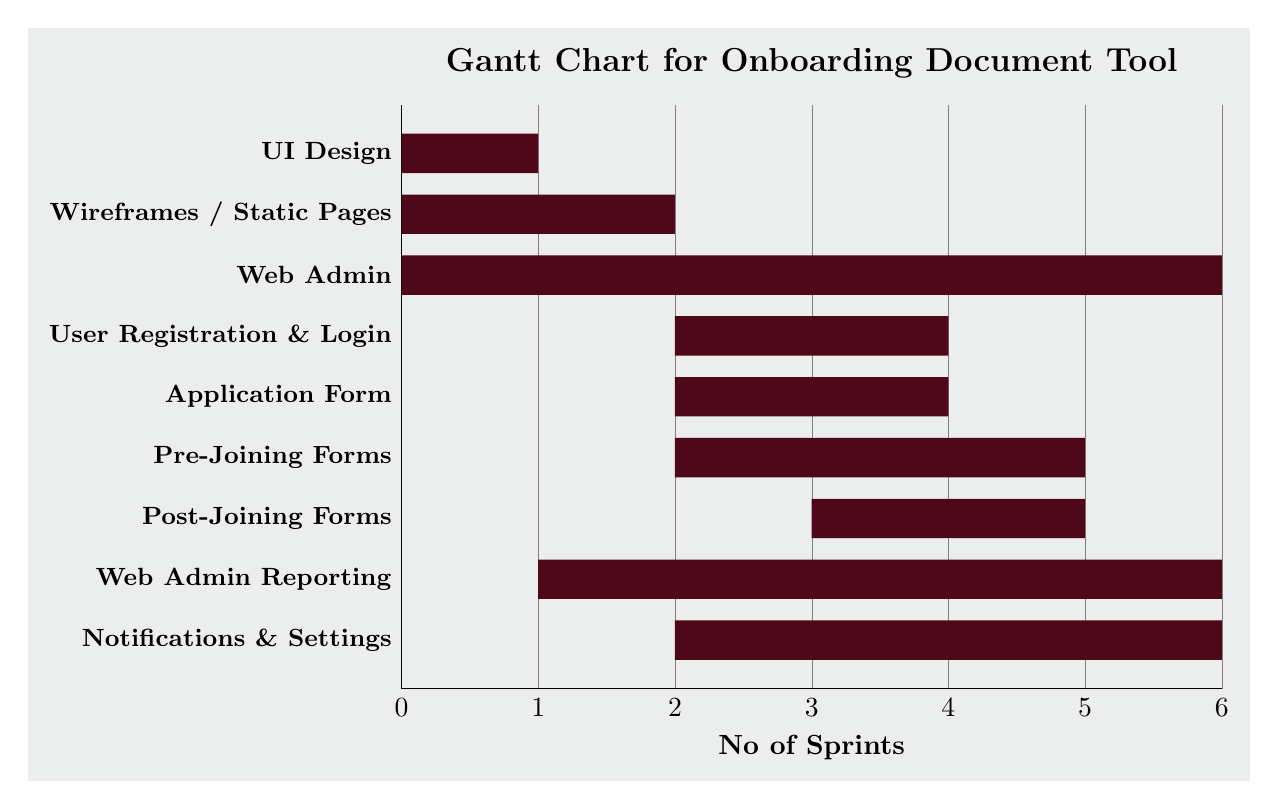
\begin{tikzpicture}[use background]
		
	
		
		\pgfplotstableread{ % Read the data into a table macro
			Label                                                      First   Second  
			{\small \textbf{Notifications \& Settings}}                  2     4    
			{\small \textbf{Web Admin Reporting}}                        1     5   
			{\small \textbf{Post-Joining Forms}}                         3     2    
			{\small \textbf{Pre-Joining Forms}}                          2     3    
			{\small \textbf{Application Form}}                           2     2   
			{\small \textbf{User Registration \& Login}}                 2     2    
			{\small \textbf{Web Admin}}                                  0     6 
			{\small \textbf{Wireframes / Static Pages}}                  0     2 
			{\small \textbf{UI Design}}                                  0     1
		}\datatable
		
		\begin{axis}[
		xbar stacked,   % Stacked horizontal bars
		xmin=0,  xmax=6,       % Start x axis at 0
		title={\large \textbf {Gantt Chart for Onboarding Document Tool}},
		height=9cm, width=12cm,
		bar width=0.5cm,
		axis x line*=bottom,
		axis y line*=left,
		y axis line style={opacity=1},
		enlarge y limits=true,
		xmajorgrids={true},
		grid style={
			solid,
			ultra thin,
			gray
		},
		tick style={tickwidth=0cm,major tick length=0cm},
		xlabel={\textbf{No of Sprints }},
		ytick=data,     % Use as many tick labels as y coordinates
		yticklabels from table={\datatable}{Label}  % Get the labels from the Label column of the \datatable
		]
		\addplot [draw=none,fill=none] table [x=First, y expr=\coordindex] {\datatable};    % Plot the "First" column against the data index
		\addplot [draw=none,fill=levelfirst]table [x=Second, y expr=\coordindex] {\datatable};
		
		
		\end{axis}
		

		\end{tikzpicture}
		

		\end{center}
		
		\noindent
		These estimates may change nominally depending on the exact nature of detailed requirements. Likewise, minor modifications would not be considered out of scope.\\ \\
		Maintenance period would start after the delivery of the final deliverable.\\ \\
		Maintenance would include fixes of any defect encountered while functioning of the application.\\ \\
		Maintenance would not include development of any new requirements / enhancements / changes in the application.
		
		\newpage
		
		\section{Tech Stack}
		
		\subsection{Back-end}
		\begin{easylist}
		 & \thinspace Java (A performance-intense and secure application development language).
		 & \thinspace Postgresql Database (Advanced Open Source Database, similar to Oracle).
		 & \thinspace Play Framework (Web Application framework).
		 & \thinspace Hosted on Linux (Ubuntu 15.04).
		 & \thinspace SSL Certification (HTTPS).
		\end{easylist}
		
		\subsection{Front-end}
		\begin{easylist}
			& \thinspace HTML 5, CSS 3, Jquery
			& \thinspace Bootstrap Framework
			& \thinspace Responsive UI which would ensure mobile-friendliness of the application
		\end{easylist}
		
		\newpage
			
		\section{High Level Architecture}	
		\begin{center}	
		\includegraphics[width=\textwidth]{Architecture.png}\\[-1em]
		\end{center}          
		
		\newpage
		
		\section{Project Cost and Maintenance}
		\begin{center}
			
			\rowcolors{2}{tablecell2}{tablecell2}
			
			{
				\setlength{\extrarowheight}{2pt}
				
				\newcolumntype{b}{X}
				\newcolumntype{s}{>{\hsize=.25\hsize}X}
				\newcolumntype{t}{>{\hsize=1.8\hsize}X}
				
			
				\begin{tabularx}{\textwidth}{s X cX t }
					
					\rowcolor{levelfirst}

					{ \textbf{\textcolor{white}{Sr. No.\newline}}} & {\textbf{\textcolor{white}{Deliverable / Module}}} & \textbf{\textcolor{white}{Cost INR}} & \textbf{\textcolor{white}{Remarks / Conditions if any}}\\
					
					1. & Web \& Server-side components & INR 4,00,000 & \\
					
					
					2. & Server/ Hosting/ SSL Charges & & @extra or to be borne by the Client  \\
					
					
					3. & Per Change Request & & @extra. Rs 10,000 per resource per day  \\
					
					\rowcolor{tablecell1}
					{ \textbf{\textcolor{levelfirst}{A.}}} & { \textbf{\textcolor{levelfirst}{Total Charges*}}} & { \textbf{\textcolor{levelfirst}{INR 4,00,000}}} & { {\textcolor{levelfirst}{Taxes not included}}}  \\
					
					4. & Maintenance Charges &  & {Free Support for the first 3 months post deployment in production \newline 20 \% of Total Charges + Applicable Taxes per year.}	\\
				\end{tabularx}
			}
		\end{center}
		\noindent
		\small {\slshape{* Total Charges are an estimate based on the High Level Understanding of the requirements stated in the RFP. Actual charges may vary depending on the effort estimation after the complete requirement details are shared and mutually agreed to. Any additional requirements shall be change requests chargeable according to the effort required.}}
		
		\newpage
		
		\section{Terms and Conditions}
		\begin{easylist}
		& \thinspace All applicable taxes are extra
		& \thinspace The IP of the application will be Customer’s property
		& \thinspace Thrymr can kick off the project within a week of receiving the PO/ WO.
		& \thinspace The Purchase Order to be released in the name of Thrymr Software Pvt Ltd.
		& \thinspace A separate Statement of Work (SOW) may be entered into if this proposal is accepted.
		& \thinspace 50\% payment shall be in advance. 50\% of the payment shall be at the project completion (production deployment or completing a sign off)
		\end{easylist}
		
		\section{Acceptance and Sign-off}
		
		Customer will provide a set of UAT test cases for each module. Against successful execution of these UAT test cases the final sign off will be given by the customer.\\ \\
		Thrymr Software and the Customer will mutually agree on user acceptance that ensures a bug free application to the satisfaction of the users and as defined in the specifications.
				
\end{document}	
	









